\documentclass[11pt,oneside]{report}
\usepackage{graphicx}
\usepackage{epstopdf}
\usepackage[letterpaper]{geometry}
\usepackage{amsmath}
\usepackage{amsfonts}
\usepackage{mathrsfs}
\usepackage{titlesec}
\usepackage{fullpage}
\usepackage{setspace}
\usepackage{bold-extra}
\usepackage{tocloft}
\usepackage{url}
%\usepackage{apacite}
\usepackage{fancyhdr}
\usepackage[free-standing-units]{siunitx}
\usepackage{multirow}
\usepackage{caption}
%\usepackage{subcaption}
\usepackage{booktabs}
\usepackage{array}
\usepackage{listings}
\usepackage{longtable}
\usepackage{enumitem}
%\usepackage{subfig}
\usepackage{placeins}

\usepackage{color}

\usepackage{caption}
\usepackage{subcaption}
\usepackage[toc,page]{appendix}

\newcommand\numberthis{\addtocounter{equation}{1}\tag{\theequation}}

\definecolor{dkgreen}{rgb}{0,0.6,0}
\definecolor{gray}{rgb}{0.5,0.5,0.5}
\definecolor{mauve}{rgb}{0.58,0,0.82}

\lstset{frame=tb,
  language=c++,
  aboveskip=3mm,
  belowskip=3mm,
  showstringspaces=false,
  columns=flexible,
  basicstyle={\small\ttfamily},
  numbers=none,
  numberstyle=\tiny\color{gray},
  keywordstyle=\color{blue},
  commentstyle=\color{dkgreen},
  stringstyle=\color{mauve},
  breaklines=true,
  breakatwhitespace=true,
  tabsize=3
}

\newcommand{\chapterStyle}{\LARGE\bfseries\scshape\centering}

\titleformat{\chapter}[hang]{\chapterStyle}{\thechapter.0}{1em}{}
\titlespacing{\chapter}{0em}{-5em}{0em}

\titleformat{\section}[hang]{\Large\scshape\bfseries}{\thesection}{1em}{}

%\titleformat{\section}[hang]{\large\bfseries}{\thechapter.0}{1em}{}

% prevents TOC from resetting page numberings
\let\oldsetcounter=\setcounter
\renewcommand\setcounter[2]{%
    \def\arg{#1}\def\pg{page}%
    \ifx\arg\pg\else\oldsetcounter{#1}{#2}\fi}
        
\renewcommand{\cfttoctitlefont}{\hfill\chapterStyle}
\renewcommand{\cftaftertoctitle}{\hfill}
\renewcommand{\cftloftitlefont}{\hfill\chapterStyle}
\renewcommand{\cftafterloftitle}{\hfill}
\renewcommand{\cftlottitlefont}{\hfill\chapterStyle}
\renewcommand{\cftafterlottitle}{\hfill}

\renewcommand\listfigurename{\centering List Of Figures}
\renewcommand\listtablename{\centering List Of Tables}
\renewcommand{\contentsname}{\centering Contents}
\renewcommand\bibname{References}
\renewcommand{\abstractname}{\vspace{-1.2cm}Executive Summary}

\newcommand{\docSpacing}{1.6}

%file, caption, label, scaling
\newcommand{\picfigure}[4]{\begin{figure}\begin{center}\includegraphics[scale = #4]{#1}\caption{#2}\label{#3}\end{center}\end{figure}}

%partial derivative
\newcommand{\partiald}[2]{\frac{\partial #1}{\partial #2}}

\makeatletter
\newcommand*{\compress}{\@minipagetrue}
\makeatother

\setlength{\headheight}{15pt}

\begin{document}

\newpage
\pagestyle{plain}
\pagenumbering{roman}
\setcounter{page}{0}

%% Title Page
\begin{titlepage}
\centering
\textsc{\LARGE Quartz Imaging Corporation}\\[0.5cm]
% Title
{ \huge \bfseries SEM Imaging Simulation\\[0.4cm] \hrule \vspace{0.4cm} \large Project 1510} \\[1em]

% Author and supervisor
\begin{minipage}{0.4\textwidth}
\begin{flushleft} \large
\emph{Author:}\\
Rey \textsc{Zeng Ruizi} 
\end{flushleft}
\end{minipage}
\begin{minipage}{0.4\textwidth}
\begin{flushright} \large
%\emph{Quartz Imaging Corporation} \\
Mr. Andrew \textsc{Brown}\\ [1em]
Mr. James \textsc{F}\\ [1em]

\end{flushright}
\end{minipage}
\vfill
\includegraphics[width=0.9\textwidth]{./img/train_title.eps}
\vfill
{\large \today}
\end{titlepage}


\setstretch{\docSpacing}
\begin{abstract}
\thispagestyle{plain}
\addcontentsline{toc}{chapter}{Executive Summary}
In order to design effective modern wireless systems, knowledge of the medium where signals propagate (the channel) is required. In particular, the statistical locations of radio wave reflectors (scatterers) in the environment is essential to evaluate and design systems. The acquisition of this data is done through devices known as channel sounders. Currently, channel sounders are large, laborious, and expensive (hundred thousand dollar range) devices.

The main goal of our project is to build and test a small and inexpensive (thousand dollar range) channel sounder that creates an image showing the exact locations of radio scatterers in the ISM band (903 -- 928 MHz), so that accurate channel models may be constructed.

The sounder consists of a stationary transmitter and a vehicular receiver. The receiver, whose positions are known at all times, captures and logs the signal. In post-processing, received data is first transformed into a ranged-compressed history. Then, a synthetic aperture radar imaging algorithm known as Back Projection is employed to recover the scatterer locations from this range-compressed history. The receiver and transmitter consist of USRPs (programmable radio transceivers), Rb clocks (for synchronization), GPS receivers (for position and time synchronization), and mini-computers for control and data storage. The channel sounder's center frequency is 915 MHz, bandwidth is 25 MHz, theoretical spatial resolution is 12 m, and costs around \$12000.

Several lab tests, including direct connection and antenna transmissions, were conducted to verify transmission and reception of signals. During static testing using antenna, the system was able to detect a 2 square-meters metal plate target at 150 m total range. However, tests also revealed drifting offset in GPS time synchronization and a bottleneck in receiver data storage. Finally, fields tests were done along a 200 m section of $16^{\text{th}}$ avenue on the west of Pacific Spirit Park in Vancouver. The received data was processed to yield an image of the target environment that corresponded reasonably well to a map of the area.

Overall, we recommend that work continue on this project, with some modifications. Current directions of improvement are investigating better position tracking using vehicle speed sensors, finding a reliable way to synchronize the transmitter and receiver, and acquiring a faster data storage medium.
\end{abstract}

\setstretch{1}
\quad\\[-6em]
\tableofcontents
\newpage
\quad\\[-6em]
\listoffigures
\listoftables
\addcontentsline{toc}{chapter}{List of Figures}
\addcontentsline{toc}{chapter}{List of Tables}

\newpage
\setstretch{\docSpacing}

\chapter*{Glossary}
\addcontentsline{toc}{chapter}{Glossary}

\renewcommand{\arraystretch}{1.5}
\begin{longtable}{>{\raggedleft\arraybackslash}p{3.5cm}p{11cm}}
\bfseries{ADC} & Analog to Digital Converter\\
\bfseries{Back Projection} & A time-domain algorithm takes advantage of the changing Doppler shift over time to map out relative locations of scatterers\\
\bfseries{Channel} & In telecommunications, the physical medium used to transmit a signal\\
\bfseries{Channel Model} & A description of a physical channel, including scatterers, distortion effects, and fading\\
\bfseries{DAC} & Digital to Analog Converter\\
\bfseries{DRGPS} & Dead Reckoning GPS, a device that combines GPS information and vehicle speed information to gauge position accurately\\
\bfseries{Fading} & When 2 signals of different phase interfere, causing destructive interference\\
%\bfseries{FSPL} & Free Space Path Loss, the attenuation of a radio signal as it travels from an isotropic radiator to an isotropic antenna via free space. The attenuation encapsulates the effect of propagation distance and the effect of the antenna \\
%\bfseries{GPGGA} & Global Positioning System Fix Data\\
\bfseries{GPS} & Global Positioning System, a network of satellites used for reckoning positioning and time. \\
\bfseries{GPSDO} & GPS Disciplined Oscillator, a highly precise (and accurate) clock. \\
\bfseries{HSR} & High speed rail \\
\bfseries{MIMO} & Multiple input multiple output, a radio technique involving sending data along different paths than the main line of sight in order to increase capacity or to work around obstructions\\
\bfseries{PPS} & Pulse-per-second signal, shared by GPSDOs acquired from the GPS system\\
\bfseries{PRBS} & Pseudo-Random Binary Sequence. A binary sequence of numbers consisting strictly of 0 and 1\\
\bfseries{Processing Frame} & A linear array that contains a pre-defined number of samples meant to be processed as a single unit.\\
\bfseries{SAR} & Synthetic aperture radar, an imaging technique that uses moving antennas to construct a scene\\
\bfseries{Scatterer} & An object that deflects a radio signal, causing multiple propagation paths\\
\bfseries{UPS} & Uninterrupted Power Supply\\
\bfseries{USRP} & Universal Software Radio Peripheral, a device with fast DACs and ADCs for radio signals\\
\end{longtable}

\renewcommand{\arraystretch}{1}
\setstretch{\docSpacing}

%reduces excessive whitespace around equations
\setlength{\abovedisplayskip}{1pt}
\setlength{\belowdisplayskip}{1pt}
\setlength{\abovedisplayshortskip}{1pt}
\setlength{\belowdisplayshortskip}{1pt}

\chapter{Introduction}
\pagestyle{fancy}
\fancyhead{}
\fancyhead[R]{\thepage}
\fancyfoot{}
\renewcommand{\headrulewidth}{0pt}
\renewcommand{\footrulewidth}{0pt}

\pagenumbering{arabic}
\setcounter{page}{1}
Driven by Moore's Law, the size of transistors has shrunk to nanometer scale. The small size of the transistors posts significant challenges for semiconductor failure analysis as it becomes increasingly difficult to obtain clear images of the device.

The most common technique to acquire images of semiconductor is scanning electron microscopy (SEM). SEM scans the object being image and collects the low energy secondary electrons, which are electrons produced from the object itself by chain reaction due to the higher energy primary electron. Several problems are presented when using this techniques to acquire images. For example, at high magnification there are significantly more electrons produced at around the edge of object to to increased surface area, which results in the edges being brighter than the rest of the object. This ``edge bloom'' effect affects the measurement of critical dimensions as it is difficult for software to identify the edge during the post procesing step. On the other hand, the boundaries between materials are unclear sometimes. These problems call for a better method for measurement.

In recent years, machine learning has proven to be a powerful end--to--end solution in many area of data science, including natural language processing and image analysis. In particular, convolutional neural network (CNN) is a useful tool in image analysis. In order to utilize this tool, a large number of labelled data are required `train' a neural network, which would perform a specific task based on the designed of the net.

It is known that a slightly worse model would out perform a more `advanced' model given the proper data \cite{halevy2009unreasonable}. However, acquiring the large number of data required for training neural network is a daunting task. Most semiconductor images are confidential properties, and annotating the images for training purpose requires tedious effects and is proned to human error. It would be convenient to generate the images programmatically, in which case an unlimited number of images can be acquired. 

JMONSEL \cite{villarrubia2015scanning}, developed by John Villarrubia and Nicholas Ritchie of NIST, is a single--threaded electron tracker written in Java. It simulates the physical interactions between electron and the surrounding materials as it traverses through the material. Using the simulation results from JMONSEL, it is possible to construct realistic electron microscope images. However, the program runs very slowly, partly due to the fact that it is written in Java. The program needs to be modified in order to generate enough images in a feasible amount of time for training neural network.

This report details the concept, construction, verification and working details of a multi-threaded, CUDA--compliant C++ version of JMONSEL, CudaMONSEL, that is able to rapidly generate the SEM images required. Initial tests shows that CUDAMONSEL is up to $5$ times faster than JMONSEL when running on a single--thread, and the number of threads are only limited by the number hardware of the device running the simulator.
\chapter{Concepts}\label{con}
The goal of project is to accurately simulate the trajectory of a electron from creation to destruction in a computational efficient manner so that large quantity of synthesized images can be obtained in feasible time to be used for training of neural networks. This section contains the background and algorithm for tracking each electron throughout its lifetime. The algorithm is being developed jointly by John S.  Villarrubia and Nicholas W. M. Ritchie of NIST.

\section{Simulation}\label{con:monte_carlo_ss}
%\begin{figure}[h]
%\begin{center}
%\includegraphics[width=0.7\textwidth]{img/Propagation_Concept.pdf}
%\caption{\label{fig:Propagation_Concept}An one-scatterer propagation environment}
%\end{center}
%\end{figure}

The simulation tracks the propagation of an electron trversing through regions. An electron is spawned by an electron gun targeted at a specific position on the material. Any activity generated by the physical interation between the electron fired and the material is attributed to the targetd location. During the propagation, the electron may interact with the material in the region, or cross the boundary between two regions. Depending on the corresponding scattering mechanisms or barrier scattering mechanism, both interaction may spawn a new electron.

\section{Material}\label{con:material}
%\begin{align*}
%   S &= \sum_{t} R_r(t,r_c(t))e^{-\frac{j 2 \pi r f_c }{c}} \\
%     &= \sum_{t}\sum_{k=1}^{N(t)} A_k(t) R_s(r_c(t)-r_k(t))e^{-\frac{j 2 \pi r f_c }{c}}
%\end{align*}
Various physical scattering models require different material properties. Material is defined by its elemental composition and density. The exact composition of the material is used to obtain 
\begin{enumerate}
\item MeanIonizationPotential in JoyLuoNieminenCSD
\item RandomizedScatterFactory (NISTMottRS Factory for example) in SelectableElasticSM etc.
\end{enumerate}

\subsection{SE Material}\label{subsec:sematerial}
SE material is an extension of material that provide more material properties for scattering models. The models can then decide which properties to use and how to use them. Additional properties made available by this extension include the material work function, plasmon energy, the location of the conduction band minimum, and electronic structure of the material in the form of a representation of the density of states.

For some models, scattering cross sections depend upon the target electron's kinetic energy and not simply upon its total energy. To facilitate these models, kinetic energies are associated with each of the states. These energies may be supplied by the user (e.g., based upon literature values or the user's own model for the material). If they are not supplied by the user, default values are supplied. For electrons in the conduction band (energy above the conduction band minimum) the default algorithm assigns a kinetic energy equal to the distance of the state above the band minimum. For electrons at lower levels the default algorithm assigns a kinetic energy equal to the distance of the state below the vacuum level. The user should override the default values if more accurate informations are available.

\section{Material Scatter Model}\label{con:msm}
A material scatter model consists of three parts:
\begin{enumerate}
\item A list of scattering mechanisms (e.g., Mott elastic scattering, Moller SE production, Plasmon SE production,...) that operate in the material. These scattering mechanisms may discontinuously (i.e., at a scattering event) change the primary electron energy and direction and they may create secondary electrons.
\item A single barrier scattering function. This method models scattering at a material interface.
\item A single continuous slowing down function. Determines the energy loss of the primary electron within the material. 
\end{enumerate}
Each material in the sample must be associated with a material scattering model. It combines the various mechanisms to determine overall scattering behavior, including free path, secondary generation, etc. 

\section{Scatter Mechanism}\label{con:sm}
A scatter mechanism is a physical event which governs the motion of electron. Each material scatter model can hold multiple scatter mechanisms, each with its own scatter effects and probability of occuring (eg. scattering rate). Its effects are a function of the medium/material and the electron's current energy. Effects can include changing the (primary) electron's direction and energy, and even generating a secondary electron with its own energy and direction through some inelastic scattering events. 

\section{Barrier Scatter Mechanism}
Barrier scattering occurs when an electron encounters a boundary between two materials. Differences in the potential energy (work function, etc.) in the two materials may cause a change in the electron's energy or trajectory. Note that it is possible for the barrier scatter mechanism to produce a secondary electron. 

The only barrier scatter mechanisms included in JMONSEL is the \emph{Exponential Quantum Mechanical Barrier Scatter Mechanism}.

\subsection{Exponential Quantum Mechanical Barrier Scatter Mechanism}
\begin{align*}
   U(x) &= \frac{\Delta U}{1+e^{-2x/\lambda}} \numberthis \label{eq:expqmsm}
\end{align*}
Quantum mechanical scattering from a finite--width barrier with ``exponential'' shape, meaning the form of the potential energy barrier is assumed to be \eqref{eq:expqmsm}. This barrier function represents a smooth `s--shaped' transition from $U(x)=0$ well to the left of the barrier to $U(x)=\Delta U$ well to the right. $\lambda$ is a measure of the width of the barrier. Roughly half (~46\%) of the transition occurs over a distance equal to lambda (from $x = -\lambda/2$ to $x = \lambda/2$), $90\%$ over $3\lambda$.

In the limit that lambda is ``large'', this probability approaches the classical result. In the limit that lambda goes to $0$, it approaches the transmission probability for sharp barriers encountered in elementary quantum mechanics texts. For most purposes the useful range of $\lambda$ values is from $0 m$ to $1e-9 m$. Anything larger than this is essentially classical.

This is therefore a somewhat general implementation of barrier scattering that includes classical and sharp-barrier quantum mechanical scattering as special cases. Two constructors are provided. Both constructors accept a material as input (from which the barrier height is determined). One constructor additionally allows specification of $\lambda$. The other does not. The constructor without $\lambda$ specification implements classical barrier scattering (the large lambda limit). This method of implementing classical barrier scattering is preferred to giving an explict but large value of $\lambda$ because it uses a simpler limiting--case formula, and it avoids possible numerical issues associated with large arguments. The constructor with an explicit $\lambda$ specification implements quantum mechanical scattering for a barrier of the specified width.

\section{Slowing Down Algorithm}\label{con:sda}
Slowing down algorithms compute energy change for an electron as a function of initial energy and distance moved. The loss depends on properties of the medium through which the electron travels.
 
\subsection{Joy--Luo--Nieminen SDA}
Implements a continuous energy loss formula modified for low energies. Above a cutoff energy it uses the Bethe energy loss as modified by Joy and Luo. The Joy/Luo modification improves the accuracy at low energies. Below the cutoff energy it approximates the energy loss as proportional to the electron's energy to the 5/2 power, as described by \cite{Nieminen}. The dividing line between these two approximations is a parameter that must be supplied to the constructor when this slowing down algorithm is instantiated. The proportionality constant in Nieminen's low energy form is then chosen to enforce equality of the two forms at the cutoff energy.

This scattering mechanism uses the following material properties, which therefore need to be properly defined: workfunction (unless supplied in the constructor), the elemental composition, density, and weight fractions.
\chapter{Implementation}\label{impl}
In this section we discuss the implementation details of CudaMONSEL.

The simulation is divided into two main packages, microanalysis and nanoanalysis, based on their respective functionalities and thus, authors. The microanalysis package, authored by Nicholas Ritchie, deals primarily with x--ray analysis, while the nanoanalysis package, authored by John Villarrubia, focuses on electron's interactions with materials. While their applications are different, nanoanalysis depends on microanalysis' implementation (mostly geometry) to work. We will introduce both sections below, with an emphasis on the connections between the two packages.

\section{Microanalysis}
In this package, the physics of the simulation are provided by subclasses of \emph{AlgorithmUser} and \emph{AlgorithmClass} abstract classes.

\subsection{Algorithm Classes}
This section is dedicated to the implementation details of classes that are related the physics of the simulation. All of these classes are derived from the abstract base class algorithm 

The main purpose of \emph{AlgorithmUser} class is to provide the abstract method \emph{initializeDefaultStrategy} which provides a function shared by its subclasses to set each class in a proper state required to run the physics. 

The secondary purpose of this class is to provide a place for the simulation to define the default algorithms to use when none is specified. This is enabled by the \emph{Strategy} class.

The \emph{AlgorithmClass} abstract class inherits from \emph{AlgorithmUser} abstract class and included more information about the source of the physics algorithm (eg author). It also provides a way to query all physical algorithms of the same type (TODO: explain CLEARLY) via the \emph{getAllImplementations} abstract method.

\subsubsection{}

\section{Simulation}\label{impl:sim}
The simulation computes the movement of the electron for each unit of time step. First, it acquires the active electron's position. From the position info, it calculates the current active region and the associated material scattering model. To obtain the position of electron at the next time step, the simulation acquires a random mean path length of the electron based on the scattering model and computes the electron's position at next time step. With the new position, the simulation obtains the next region, moves the electron and decreases its energy. Finally, it perfoems a check to determine if the active electron's trajectory is completed. If the trajectory is not completed, the simulation performs one of three actions based on the next region. At each time step, the energy loss and position of the electron is updated. When a new electron is spawned, the original electron is stored on a stack until the new electron is destroyed when its energy falls below the tracking threshold of the scattering mechanism. Refer to function \emph{takeStep} in MonteCarloSS.cu for details. 

\section{Material}\label{impl:mat}
\subsection{Material}
\subsection{Secondary Eleectron Material}

\section{Barrier Scattering Mechanism}\label{impl:barrier_sm}
\begin{lstlisting}[caption={BarrierScatterMechanism.cuh},label={lst:barrierSM},numbers=left,escapeinside={@}{@}]
class BarrierScatterMechanism
{
public:
   virtual ElectronT* barrierScatter(ElectronT* pe, const RegionBaseT* nextRegion) const = 0;
};
\end{lstlisting}

The barrier scatter mechanism follows the abstract class shown in \ref{lst:barrierSM}.

\subsection{Exponential Quantum Mechanical Barrier Scatter Mechanism}
A barrier scattering mechanism is associated with each region of our sample, but barrier transmission is a pair-wise phenomenon. That is, the barrier height and width at an interface between materials A and B depends in principle upon the properties of both materials. If the electron starts inside material A, then it is material A's barrier scatter mechanism that governs that particular scattering event. The present scatter mechanism determines the barrier height by comparing the potential energies in the materials on each side of the interface. It uses the barrier width associated with material A. This scattering mechanism uses the property energyCBbottom, which therefore need to be properly defined for the materials on both sides of the interface.

This class computes barrier transmission using the formula provided by \cite{Landau}. Note that this is the only barrier SM available in the JMONSEL package. 

\section{Scatter Mechanism}\label{impl:sm}
\begin{lstlisting}
class ScatterMechanism
{
public:
   /**
    * Returns the reciprocal of the mean free path.
    *
    * @param pe - the primary electron
    * @return double Reciprocal of mfp in inverse meters
    */
   virtual double scatterRate(Electron pe) = 0;

   /**
    * Updates properties of the primary electron based on results of scattering and returns either a secondary electron or null.
    * @param pe -- the primary electron
    * @return Electron -- the generated secondary electron or null
    */
   virtual Electron scatter(Electron pe) = 0;

   /**
    * Sets the material within which the electron scatters. This method typically precomputes and caches combinations of material properties required by the scattering model.
    * @param mat
    */
   virtual void setMaterial(Material mat) = 0;
}
\end{lstlisting}

Scatter mechanisms included in JMONSEL are:
\begin{enumerate}
\item BrowningMottElasticSM
\item FittedInelSM
\item GanachaudMokraniPhononInelasticSM
\item GanachaudMokraniPolaronTrapSM
\item KoteraPlasmonInelasticSM
\item MollerInelasticSM
\item SelectableElasticSM
\item TabulatedInelasticSM
\end{enumerate}

\section{Randomized Scatter}
The type of randomized scatter depends on the the energy of the electron.

\subsection{CzyzewskiMottCrossSection}
\subsection{BrowningEmpiricalCrossSection}
Browning empirical cross section is applicable to low energy (\<100eV) electrons. 
\begin{align*}
   CS(Z, e) &= \frac{3e-22 Z^{1.7}}{e + 0.005 Z^{1.7} \sqrt{e} + 0.0007 Z^{2} / \sqrt{e}}
\end{align*}
where $e$ is electron energy in keV, $Z$ is the proton number of the element.

\begin{align*}
    SA(Z, e)= 
\begin{cases}
    acos\left (1.0 - \frac{2.0 \alpha r_2}{\alpha - r_2 + 1}\right ),& \text{if } r_1 \leq \frac{r}{r+1}\\
    acos(1-2.0r_2),& \text{otherwise}
\end{cases}
\end{align*}
where $\alpha = 7.0e-3/e$, $r_1, r_2 \text{are random numbrs} \in \[0, 1\]$, and $r = (300.0 * e / Z) + (Z^3 / 3.0e5 * e)$.

\subsection{ScreenedRutherfordScatteringAngle}
Browning empirical cross section is applicable to high energy (\>20keV) electrons. 
\begin{align*}
   CS(Z, e) &= \frac{7.670843088080456e-38 zp (1.0 + z)}{e + 5.44967975966321e-19 zp^2}
\end{align*}
where $e$ is the electron energy in keV, $Z$ is the proton number, and $zp = Z^{1.0/3.0}$.

\begin{align*}
    SA(Z, e) &= acos\frac{1 - 2.0 * alpha * r}{1 + alpha - r}
\end{align*}
where $\alpha = 5.44968e-19 Z^{2.0 / 3.0} / e$, $r \text{is a random numbrs} \in \[0, 1\]$.

\subsection{NISTMottScatteringAngle}
\subsection{NISTMott}
NISTMott randomized scatter tries to provide a comprehensive model for all energy ranges. For low energy, it uses the Browning empirical scattering angle while for high energy, the screened Rutherford scattering angle. For energy between $100eV$ and $20keV$, it interpolates from a table built with the NIST SRD 64 method (TODO??) with Lagrange interpolation.

\begin{appendices}
\chapter{Lagrange Interpolation}
Given $n+1$ points $(x_0, y_0)$, ... $(x_n, y_n)$, the Lagrange Interpolation is given by 
\begin{align*}
    f_n(x) = \sum^{n}_{i=0} L_i(x)f(x_i)
\end{align*}
where $f(x_i) = y_i$ and $L_i(x)=\prod_{j=0,j\ne i}^{n}\frac{x-x_j}{x_i-x_j}$.
\end{appendices}

NISTMottScatteringAngle uses 2nd order interpolation in $log(E)$ for the totalCrossSection calculation. For randomScatteringAngle it uses 0th order interpolation (i.e., it chooses the nearest tabulated value) in $log(E)$ and 1st order in the random number. In contrast the present class uses 3rd order for all interpolations. Orders can be set by the constants \textit{qINTERPOLATIONORDER} and \textit{sigmaINTERPOLATIONORDER}.

$mSpwem$ is a 1--d table of total cross sections, uniform in $log(E)$ from $log(50.)$ to $log(20000)$
$mX1[j][i]$ is a 2--d table of $q$ vs $Log(E)$ and random \#. $j$ indexes $log(E)$. $i$ indexes $r$. $q$ is related to $cos(\theta)$ by $1-2q^2=cos(theta)$.

\begin{align*}
   CS(Z, e) =
   \begin{cases}
      \text{browning SA}, \text{if } e \lt 
   \end{cases}
\end{align*}
where $e$ is electron energy in keV, $Z$ is the proton number of the element.

\begin{align*}
    SA(Z, e)= 
\begin{cases}
    acos\left (1.0 - \frac{2.0 \alpha r_2}{\alpha - r_2 + 1}\right ),& \text{if } r_1 \leq \frac{r}{r+1}\\
    acos(1-2.0r_2),              & \text{otherwise}
\end{cases}
\end{align*}
where $\alpha = 7.0e-3/e$, $r_1, r_2 \text{are random numbrs} \in \[0, 1\]$, and $r = (300.0 * e / Z) + (Z^3 / 3.0e5 * e)$.

\section{Slowing Down Algorithm}\label{impl:sda}
\begin{lstlisting}
public interface SlowingDownAlg {
   /**
    * Sets the material for which the energy loss is to be computed
    *
    * @param mat
    */
   void setMaterial(SEmaterial mat);

   /**
    * compute - Computes the energy change for an electron with initial energy
    * eK traversing distance d. The return value is negative if the electron
    * loses energy.
    *
    * @param d double -- the distance moved by the electron
    * @param pe Electron, the primary electron
    * @return double -- the energy change
    */
   double compute(double d, Electron pe);
}
\end{lstlisting}
\subsection{Joy--Lou--Nieminen}

\section{Events}\label{impl:events}
The event listener `hooks' onto the simulation and provides a way to transfer information out of the simulation loop. This means that event listeners are by design passive and unable to affect the outcome of the simulations. The simulation will work even when all event--related code are removed, in which case some other mean of acquiring simulation state needs to be implemented if one wishes to retrieve any information about the on--going simulation.

The following events are defined inside $MonteCarloSS$ class:
\begin{enumerate}
\item ScatterEvent
\item NonScatterEvent
\item BackscatterEvent
\item ExitMaterialEvent
\item TrajectoryStartEvent
\item TrajectoryEndEvent
\item LastTrajectoryEvent
\item FirstTrajectoryEvent
\item StartSecondaryEvent
\item EndSecondaryEvent
\item PostScatterEvent
\item BeamEnergyChanged
\end{enumerate}

\subsection{Detector}\label{subsec:detector}
The most important events of are events relating to detecting backscattered electrons. Detectors are devices that collect the information about electrons for later processing. In the simulation, electrons that are characterized as secondary electrons are backscattered electrons with energy below $50 eV$. To simulate the detector, backscatter events are used. Backscatter events are fired only when the electron hits the chamber wall (one of the three normal end states of a electron). If required, we may also obtain forward--scattered secondary electrons for TEM image simulations.

Concretely, the event listener must be added to the simulation class (ie $MonteCarloSS$), before the start of the simulation, and have member function $actionPerformed$ of the listener classes added to the simulation deal with the appropriate events. Note that, the simulation broadcasts the event triggered to all listener classes by calling the member function $actionPerformed$ of every listener class added to the simulation in the function $fireEvent$.

\section{Amphibian -- custom C++ library}
Since one of the goals of the project is to make MONSEL compiler--independent, we built a custom library to minimize dependence on the C++ standard template library (STL). The following data structures are included,
\begin{enumerate}
\item linkedlist (single-- and double--linked)
\item vector
\item stack
\item unordered set
\item unordered map
\item (mutable) string
\end{enumerate}

Algorithms like quick sort, binary search are also included. There is also a random class responsible for generating random numbers reliably.

\chapter{System Verification}\label{sec:verify}
A variety of tests were implemented to ensure the correctness of both data imported and computation.
\begin{enumerate}
   \item Bench tests aiming to identify effects brought about by the channel sounder hardware.
   \item Stationary ranging tests aiming to verify the channel sounder's ranging capability. 
   \item Road test aiming to verify the DRGPS' position accuracy over the upcoming test campaign's terrain.
\end{enumerate}

\section{Bench Tranmission Tests}\label{sec:Verification_BenchTests}

\section{Stationary Ranging}

\subsection{Stationary Ranging A}

\subsection{Stationary Ranging B}

\subsection{Power Amplified Stationary Ranging Tests}

\section{DRGPS and Speed Sensor Accuracy Test}
\chapter{Working Details}

The main simulation loop is defined in the \textit{MonteCarloSST} class. To run the simulation, user has to provide the electron gun and the chamber as parameters to the simulation. The electron gun provides information of the initial electron where as the chamber contains the scene to be simulated. At any step of the simulation, only a single electron is being tracked as it traverses through the regions. In the case where secondary electron is spawned, the simulation saves the state of the primary electron on a stack and allow the secondary electron to take over until the secondary electron's trajectory is completed before it resumes simulating the primary electron. 

As soon as the electron leaves the electron gun, the simulation determines the next position of the electron by calculating the mean free path of the electron given the current state of the electron inside the surrounding material. As the electron moves, it loses energy. Once the electron's energy falls under the tracking energy of the material, the electron's trajectory is ended. Otherwise, the electron can be found in one of the following situations.

\begin{enumerate}
    \item The electron stays in the same region as the region before the step is taken
    \item The electron crosses a barrier from one region to another
\end{enumerate}

If either of the above applies, the electron's trajectory is ended. Note that in either situations, it is possible for a secondary electron to spawn. These are the only way a secondary electron can possibly be spawn. The probability of spawning a secondary electron is determined by the material scatter model of the material. For detail see \textit{takeStep} method in \textit{MonteCarloSS} class.

\chapter{Analysis}

\section{Backscattered Electron Energy Distribution}
In SEM imaging, we are interested in only the low energy, backscattered electrons. A large percentage of these electrons are secondary/Auger electrons spawned by the higher energy primary electron. As a result, It would be useful to study the energy distribution of the backscattered electrons to better defined the energy threshold for these secondary electrons. In this section, we examine the backscattered electron energy distribution used to produced the image on figure \ref{fig:base}. Also note that since the exact electron generation may be beyond `secondary', it is common for total electron yield to be more than $200\%$. 
\begin{figure}[h]
\begin{center}
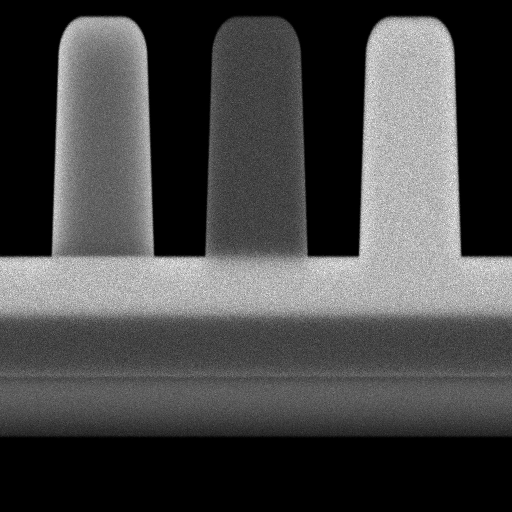
\includegraphics[width=0.5\textwidth]{img/output0.png}
\caption{\label{fig:base}SEM image of a feature with 3 lines}
\end{center}
\end{figure}

The image on figure \ref{fig:base} is generated by with primary electron energy of $1000eV$, beam radius of $0.5nm$ and $200$ electron per location using PMMA, Si and SiO2 as feature materials (left to right) while assume secondary electron energy being below $50eV$. Figure \ref{fig:bse_energy} below shows the energy distribution of backscattered electron at a particular, non--vacuum location on the image. Most of the backscattered electrons detected were low energy electrons, with a small number of of higher energy electrons detected beyond $50eV$. As a result, we conclude that it is safe to categorize electrons with energy lower than $50eV$ as secondary electrons for SEM imaging.
\begin{figure}[h]
\begin{center}
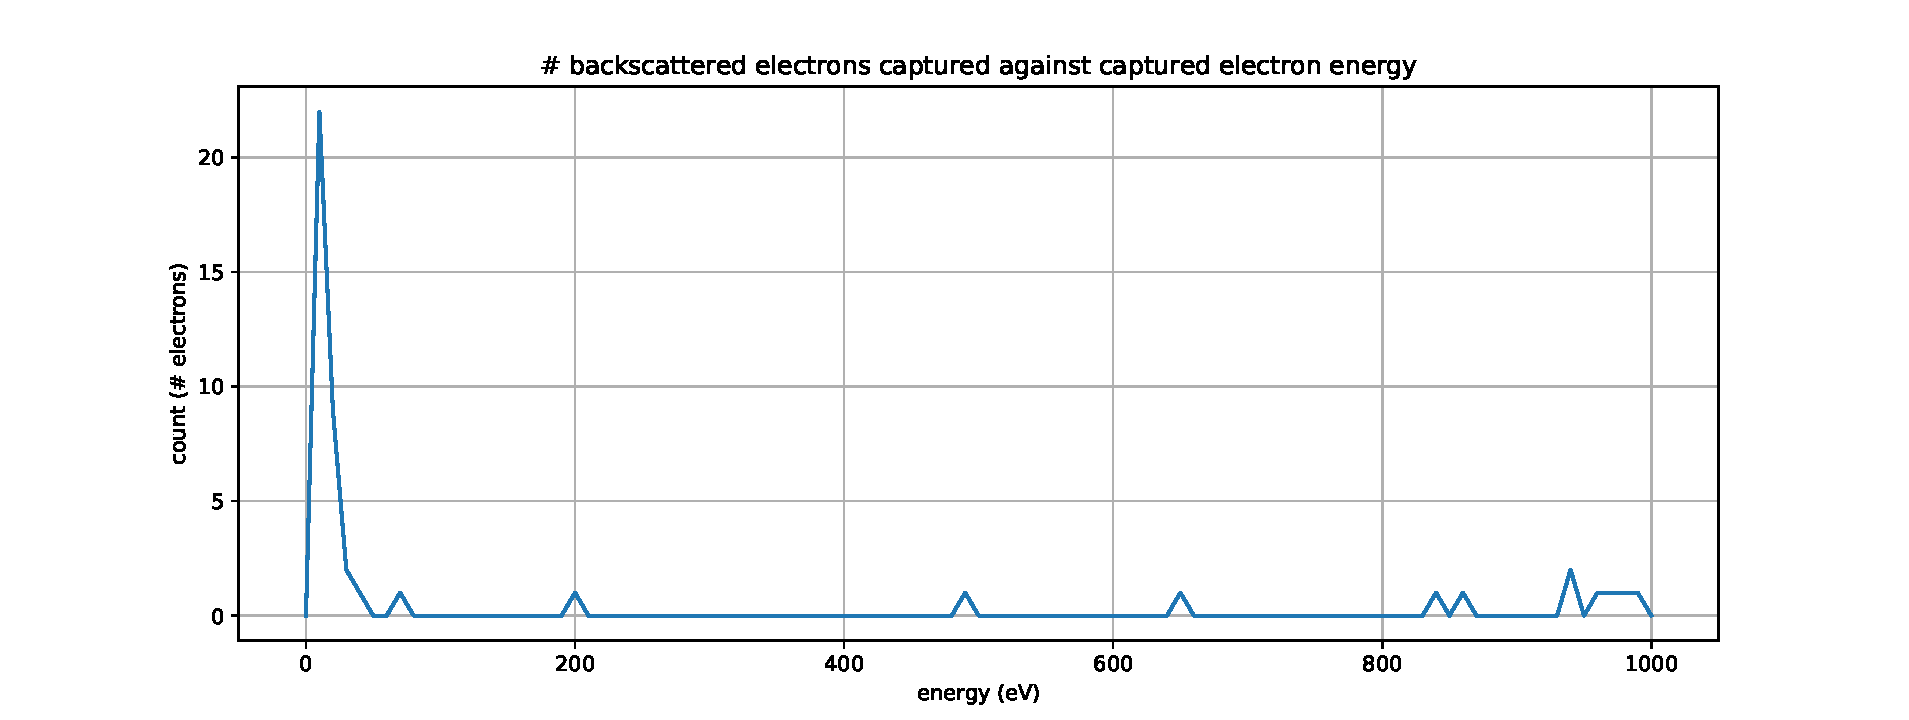
\includegraphics[width=1.0\textwidth]{img/backscattered_energy.pdf}
\caption{\label{fig:bse_energy}Backscattered electron energy distribution on a random, non--vaccum location of the image}
\end{center}
\end{figure}

To show that figure \ref{fig:bse_energy} is a representative energy distribution plot at any non--vacuum location, we produced a heat map of electron energies by acquiring a line scan of non--vacuum locations in figure \ref{fig:bse_heatmap}. The top and bottom rows of figure \ref{fig:bse_heatmap} corresponds to row 16, column 75 and 132 (left and right edges of the feature) on the image \ref{fig:base}. Since similar distributions are observed on different non--vacuum parts of the image, we will assume the distribution in \ref{fig:bse_energy} is a reasonable estimate of the energy distribution at any non--vacuum location.

\begin{figure}[h]
\begin{center}
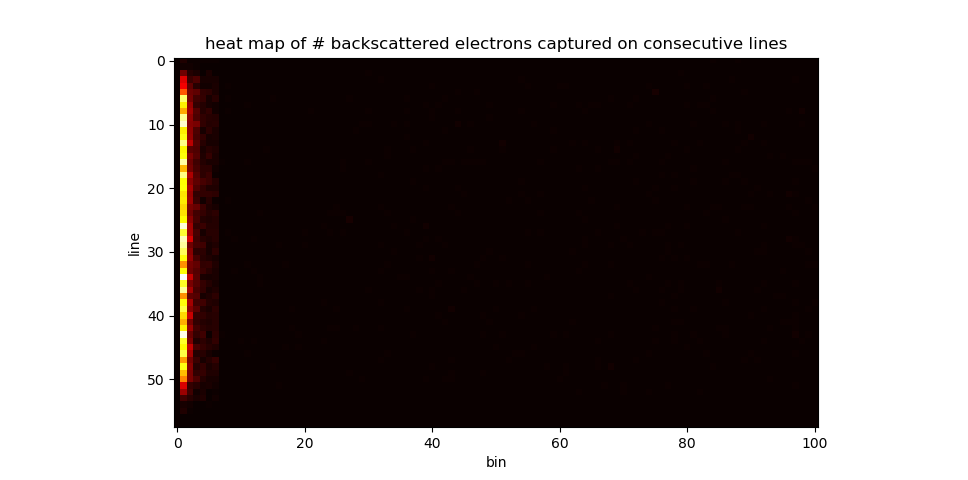
\includegraphics[width=1.0\textwidth]{img/bse_heatmap.png}
\caption{\label{fig:bse_heatmap}Heatmap of backscattered electron energy distribution on a random, non--vacuum line of the image}
\end{center}
\end{figure}

\section{Primary Electron Energy}
In the previous section, we examined the energy distribution of detected electrons and discovered that most detected electrons are SEs with low energy $<50eV$. It would be interesting to find out the effects of different primary electron energy on the SE energy distribution. In this section, we study how the primary electron energy affects the SE yield by comparing the relative quantity of SEs detected when similar electron beams are targetd on three different materials: SiO2, Si, and PMMA.

In this experiment, we used $250$ primary electrons with beam size $.5nm$ and energy of $500eV$ at each location for the first image, and increased the PE energy by $500eV$ for each subsequent image. On every image, there are 3 line features made from PMMA, Si, and SiO2 (left to right), and 3 strips made from SiO2, Si, PMMA (top to down).

\begin{figure}[h]
\begin{center}
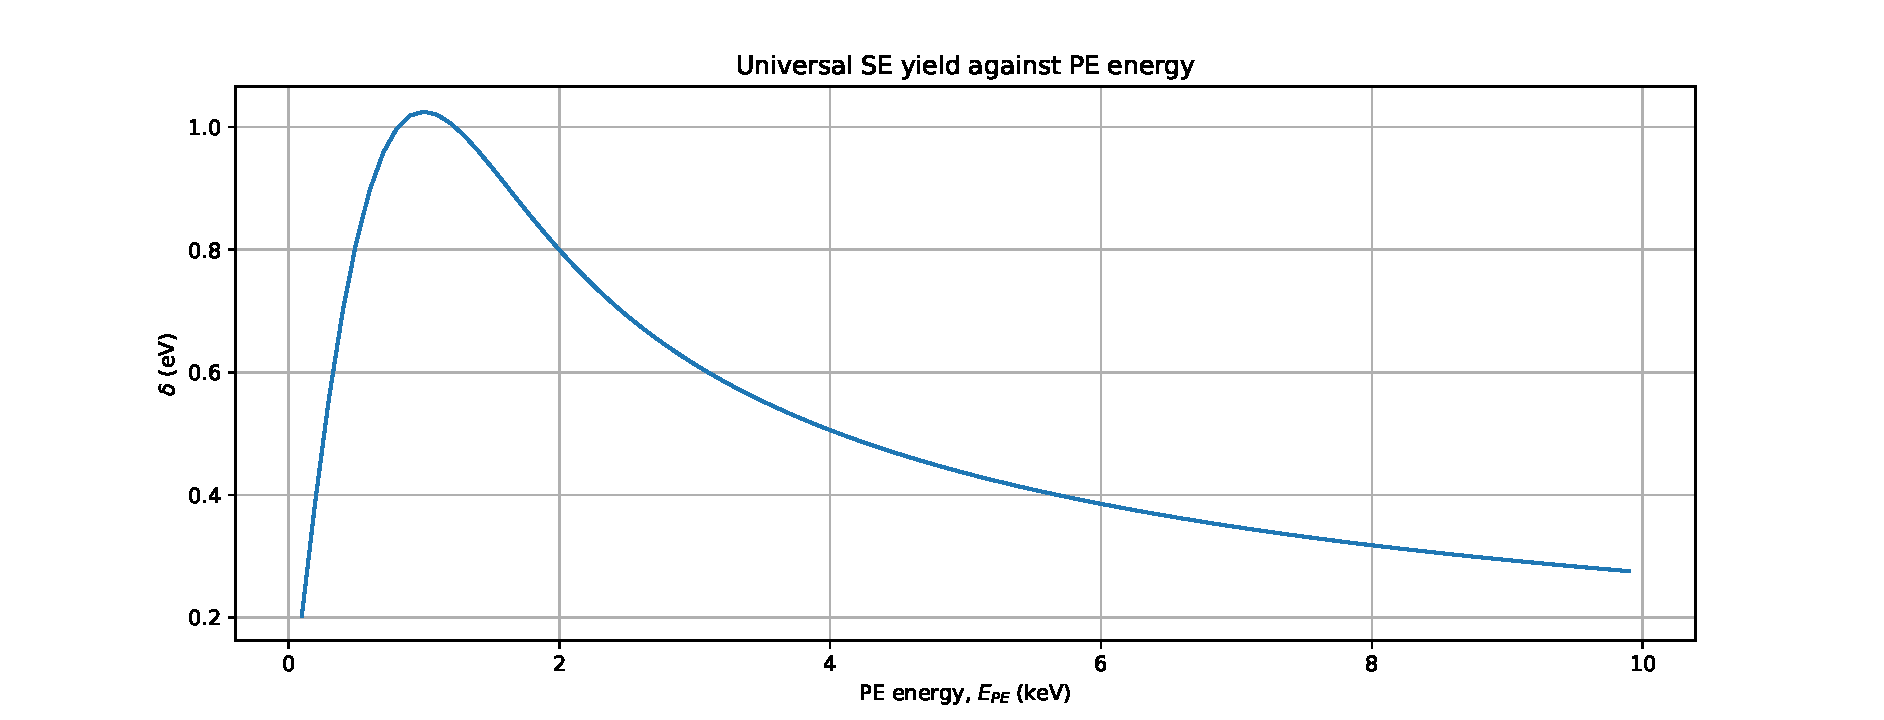
\includegraphics[width=1.0\textwidth]{img/law.pdf}
\caption{\label{fig:se_law}Universal law of SE yield against PE energy\cite{lin_newexam}}
\end{center}
\end{figure}

From the results \ref{fig:diff_beam_energy}, we can clearly see that brightness of all three materials decreased with higher energy. In particular, the relative brightness of Si decreased significantly relative to the other 2 materials, followed by PMMA while that of SiO2 remained approximately the same. The decrease in brightness in all 3 materials is consistent with the ``universal law of SE yield'', given in \cite{lin_newexam} by the equation \ref{eq:se_law} and figure \ref{fig:se_law}

\begin{figure}
\centering
\begin{subfigure}{.5\textwidth}
  \centering
  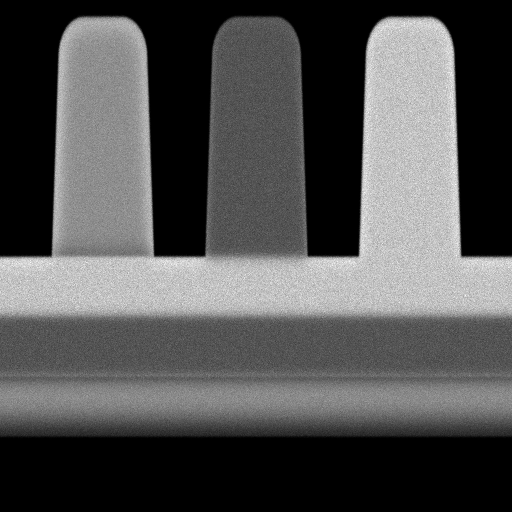
\includegraphics[width=.75\linewidth]{img/500eV.png}
  \caption{500eV beam energy}
  \label{fig:500eV}
\end{subfigure}%
\begin{subfigure}{.5\textwidth}
  \centering
  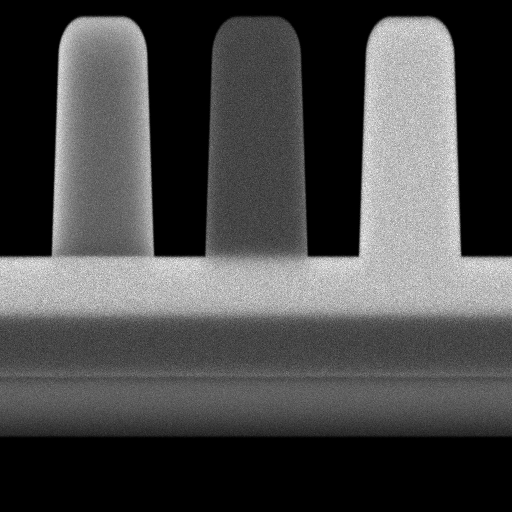
\includegraphics[width=.75\linewidth]{img/1000eV.png}
  \caption{1000eV beam energy}
  \label{fig:1000eV}
\end{subfigure}
\caption{2 images with same setup using different beam energy}
\label{fig:diff_beam_energy}
\end{figure}

\begin{align*}
   \frac{\delta}{\delta^m} &= 1.28\left(\frac{E_{PE}}{E_{PE}^m}\right)^{-0.67}\left(1-exp\left(-1.614\left(\frac{E_{PE}}{E_{PE}^m}\right)^{1.67}\right)\right) \numberthis \label{eq:se_law}
\end{align*}

where $\delta^m$ is the maximum yield, which we assumed to be 1 and $E_{PE}^m \approx 1keV$ is the primary energy of the electron where the maximum is obtained. In particular for Si, the change in brightness shows that its SE yield reaches a maximum at a few hundred electron volts and decreases monotonically at approximately $1/E_{PE}$\cite{lin_newexam} as the energy increases \cite{francesc_conventional}\cite{walker_see}.

\section{Gaussian Beam Radius}
\section{Number of Electron Trajectory per Location}
\chapter{Conclusion}
Overall, a working prototype of a spatial channel sounding device consisting of USRPs, mini-computers, GPS receivers, and atomic clocks was constructed. It used bi-static SAR algorithms to reconstruct the locations of scatterers in a field test. It has a spatial resolution of 12 m, and costs much less than current channel sounding solutions (around \$12000 in total, see Table \ref{tab:total_cost}, versus the \$100,000+ devices currently used). It is not without operational issues and difficulties however, so future work should continue on this project to make it commercially viable.
%In our first milestone, we have assembled a working setup consisting of a transmitter and a receiver from USRPs, GPSDOs, Mini-PCs and UPS. For our second milestone, we successfully identified a scatterer (Kaiser wall) using by transmitting a known signal and examine the time delay of the signal peak with respect to the line of sight peak. In our third milestone, we collected enough data during our field campaign and successfully reconstructed a scene on 16th ave. Overall, the project is a success.

\chapter{Deliverables}
The main deliverable is a working spatial channel sounding prototype, already in the Radio Science Lab. It consists of the following components.
\section{Hardware}
\subsection{Transmitter}
   \begin{itemize}
   \itemsep-1em 
      \item Mini-PC
      \item USRP
      \item Rubidium Frequency Standard
      \item GPS Receiver
      \item UPS
      \item Antenna
      \item Antenna Mast
      \item Amplifier
   \end{itemize}
\subsection{Receiver}
   \begin{itemize}
   \itemsep-1em 
      \item Mini-PC
      \item USRP
      \item Rubidium Frequency Standard
      \item GPS Receiver
      \item UPS
      \item Antenna
      \item Antenna Mount for Dr. Michelson's car
   \end{itemize}
\section{Software}
   \subsection{Transmitter}
      \begin{itemize}
      \itemsep-1em 
         \item \texttt{transmitter\_matlab.m}, Transmitter signal senerator (MATLAB)
         \item \texttt{transmitter.sln}, USRP transmitter software (C++)
      \end{itemize}
   \subsection{Receiver}
      \begin{itemize}
      \itemsep-1em 
         \item \texttt{verifySignal.m}, for verifying signal validity (MATLAB)
         \item \texttt{receiver.sln}, USRP receiver (C++)
      \end{itemize}
   \subsection{Post-Processing and Image Reconstruction}
      \begin{itemize}
      \itemsep-1em 
         \item \texttt{prepSignalForSim.m}, for range-compressing received signals (MATLAB)
         \item \texttt{jeppler\_hsrsar\_backproj.m}, Simulation and image reconstruction algorithm received from MDA.
         \item \texttt{backscatter.sln}, Fast image reconstruction algorithm re-written in C++ using DirectX and GPU.
      \end{itemize}
\section{Documentation}
   \begin{itemize}
   \itemsep-1em
      \item GPU programming concepts and documentation of our reconstruction algorithm.
      \item Proposal
      \item Final Report
   \end{itemize}
\section{Estimated Raw Cost}
Since all of these components were already available in the RSL at the time of project commencement, there are no current project costs. Table \ref{tab:total_cost} shows the estimated total cost of all parts for both the transmitter and receiver.

\begin{table}[h!]
\begin{center}
\begin{tabular}{l|l}
Item & Cost \\ \hline
2x Lenovo M93p & 2x \$800 \\
2x USRP N210 & 2x \$1700 \\
2x Rubidium Frequency Standard & 2x \$1500 \\
2x UPS & 2x \$100 \\
2x Timing GPS & 2x \$200\\
2x Panel Antenna & 2x \$200 \\
30W Amplifier & \$3000 \\
DRGPS & \$400 \\\hline
Total Cost & \$12400
\end{tabular}
\end{center}
\caption{\label{tab:total_cost} Estimated total cost of prototype system}
\end{table}

\chapter{Recommendations}
To further enhance the speed of the simulation, we may purchase a CPU that better supports multi--threading. AMD CPUs, Ryzen in particular, is better suited for this tasks than Intel CPUs historically.

Another way would be to refactor the simulation enough so that they can be ran on GPU using CUDA. The advantage would be that we would be able to speed up the simulation significantly with our existing setup. The difficulty is that due to single core optimization implemented by some of the classes, it is required for every thread to have its own copy of the entire setup. In the CUDA environment where on--board memory comes at a premium, this would require some major code refactoring and testing before any development can take place, and it may not be as cost--efficient as getting a new CPU which may also provide significant speed improvement. Having multiple GPUs enabled also proved to destabilize the Windows 10 system on our current setup, causing the system to crash by DPC\_WATCHDOG\_VIOLATION.

\bibliography{refs}
\bibliographystyle{plain}

\end{document}
